\documentclass[herrin-thesis.tex]{subfiles}
\begin{document}

\chapter[Liquid Xenon for Double Beta Decay Experiments]{Liquid Xenon for Double Beta Decay Experiments}
\chaptermark{Liquid Xenon for \(\beta\beta\) decay experiments}
\label{ch:liquidxe}

\section{Double Beta Decay Isotopes}
For nuclei with even mass number \(A\), elements with odd atomic number \(Z\) have unpaired nucleons, which is less energetically favorable than elements with even \(Z\). For some even values of \(A\), then, there exist two nuclei that differ by \(\Delta Z = 2\) that are each stable against \(\beta^{\pm}\) decay. This is depicted in \cref{fig:xe_nuclei_masses}. However, one of these nuclei will have a lower mass than the other, and so double beta decay, as described in \cref{sec:nu_doublebetadecay}, or the analogous double electron capture or double positron decay can proceed. Thirty-five naturally occurring isotopes have this property and can undergo double beta decay.

\begin{figure}[htp]
\centering
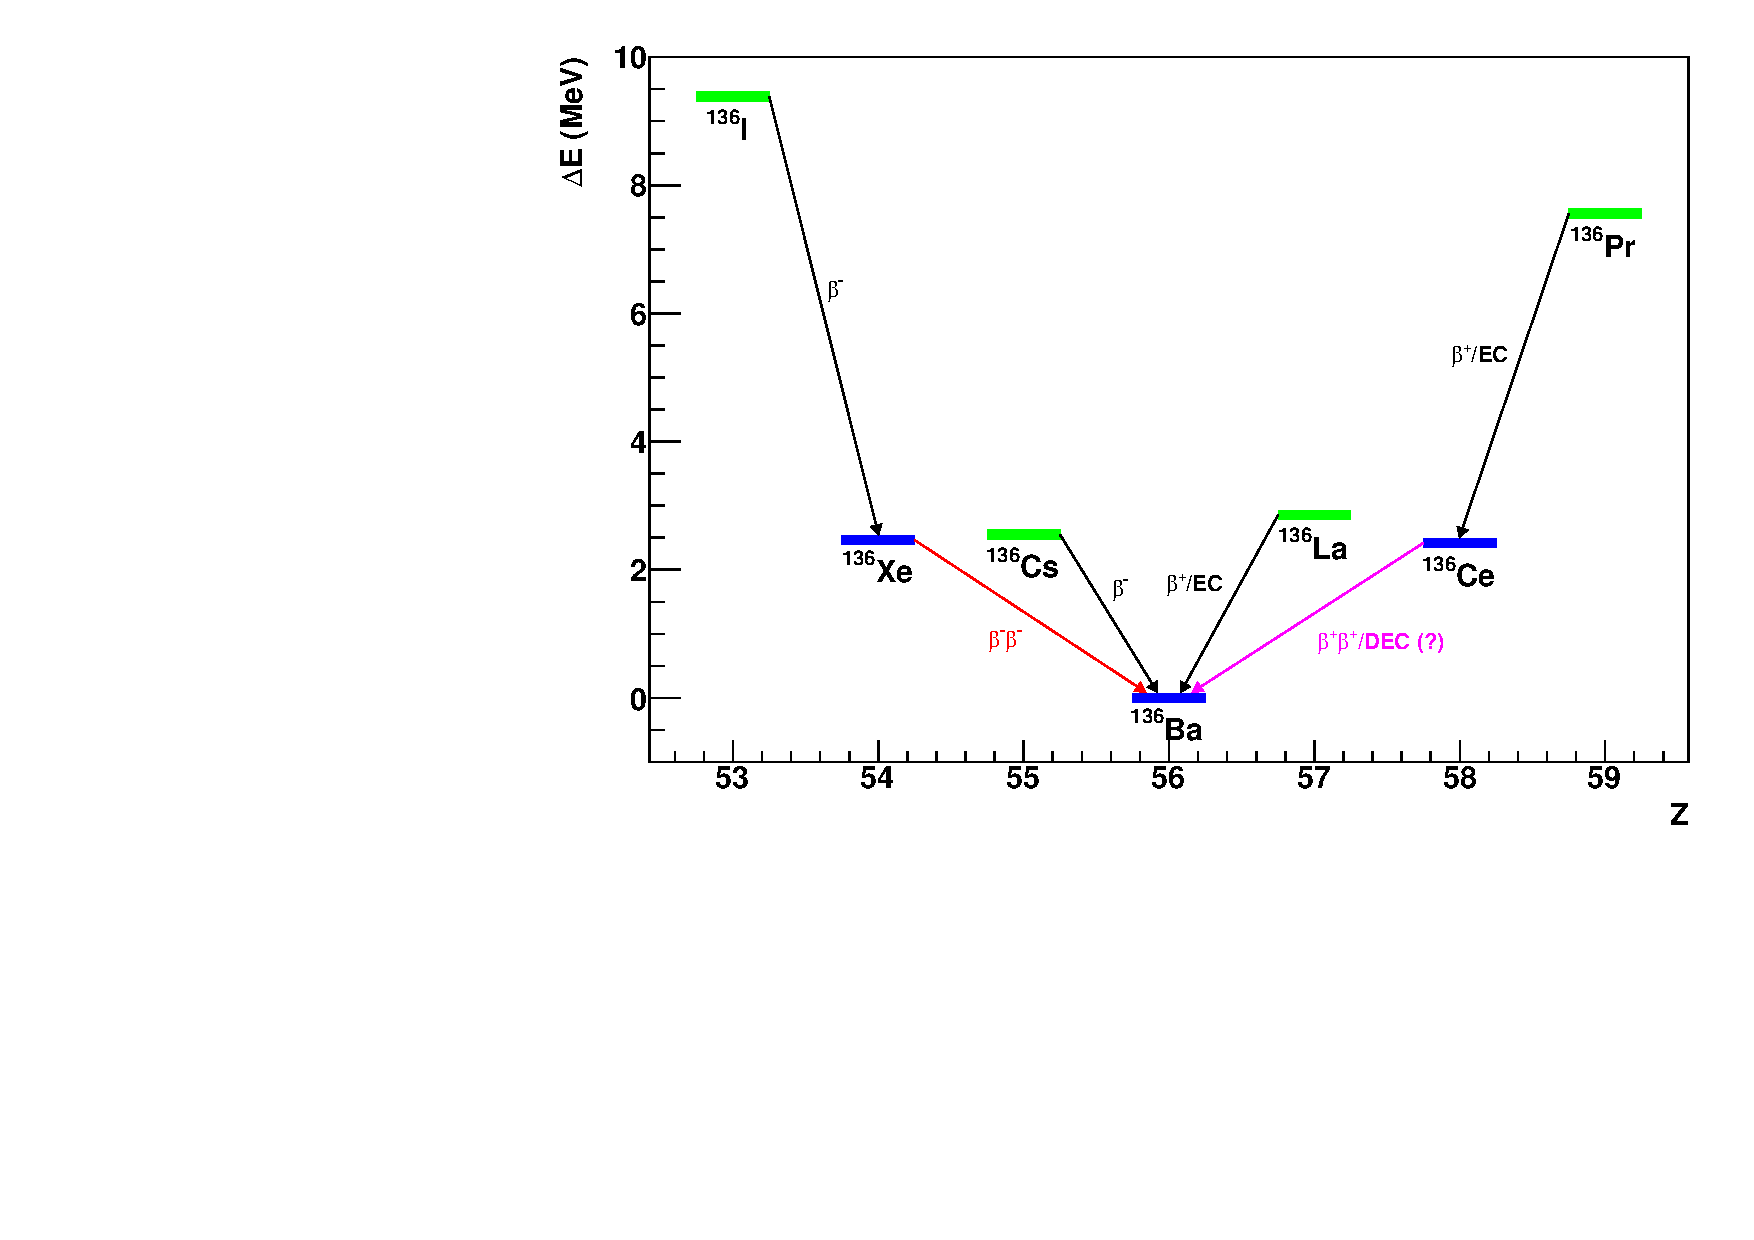
\includegraphics[width=0.6\textwidth]{./plots/xe_nuclei_masses.pdf}
\caption[Nuclear decay structure for \(A=136\)]{Nuclear decay structure for nuclei with \(A=136\). \xenon{136} is an even-even nucleus and is energetically forbidden to beta decay to \isotope{136}{Cs}. Instead, it double beta decays to \isotope{136}{Ba}. \isotope{136}{Ce} should also decay to \isotope{136}{Ba} by double \(\beta^{+}\) decay and double electron capture. However, this has not yet been observed.}
\label{fig:xe_nuclei_masses}
\end{figure}

An ideal isotope for a double beta decay experiment would be abundant. It would also have a high \(Q\) value. Higher \(Q\) value decays proceed at a faster rate. Furthermore, higher \(Q\) values place the decay energy above that of some natural sources of radioactivity, reducing backgrounds. Finally, it would be easy to use in a low radioactive background detector. Unfortunately, no single isotope is ideal, though several still have many of these favorable qualities. Having several choices is good, because if neutrinoless double beta decay is detected, it will be important to confirm this detection in other isotopes. Furthermore, the decay rate (\cref{eq:nu_zeronu_rate}) depends on nuclear matrix elements which must be estimated and have roughly a factor of 2 uncertainty for most isotopes. This means observation in multiple isotopes would be needed to precisely infer neutrino properties.

\section{The Choice of Xenon}
Ultimately, of the available isotopes, EXO has chosen to focus on xenon. Both \xenon{134} and \xenon{136} should double beta decay, though \xenon{136} has a higher Q value of \SI{2457.8}{\keV} \cite{Redshaw:2007cr}. Xenon has many properties that make it desirable for a double beta decay experiment:
\begin{itemize}
\item First and foremost, xenon can serve as both as the source and detector of double beta decay events. Noble gases and liquids have been deployed as radiation detectors for decades. A monolithic detector minimizes the other materials needed to build the detector that might be sources of radioactive backgrounds. Electrons from the double beta decay do not have to pass through other media before reaching the detector, allowing fewer energy losses and better energy resolution.
\item The Q value for \xenon{136} decays is higher than most \(\gamma\) rays from common radioactive nuclides. \isotope{208}{Tl}, which occurs on the thorium chain and emits a \SI{2615}{\keV} gamma ray, and \isotope{214}{Bi}, which occurs on the uranium chain and emits a \SI{2469}{\keV} gamma ray are notable exceptions. \(\gamma\) rays with higher energies than the Q value can potentially deposit part of their energy in the detector before scattering out, creating an event with energy close to the Q value.
\item The natural abundance of \xenon{136} is 8.9\%. Furthermore, xenon is a gas at standard temperatures and pressures, making it simple to process and enrich in \xenon{136} using ultracentrifugation.
\item Xenon is a noble element, and so it is relatively easy to purify of all chemically active contaminants. Furthermore, this purification can be done continuously by recirculating the xenon.
\item The isotopes formed in xenon by cosmogenic activation are short-lived, so the xenon only needs a short period underground and a chemical purification before it is ready to be used.
\item Xenon can be easily reused and transferred between experiments. This allows the opportunity to use xenon in complimentary or novel detector designs. Smaller experiments can help amortize the cost of larger experiments.
\item The barium daughter ion could potentially be tagged, reducing backgrounds immensely. (This technique, however, is not used in EXO-200.)
\end{itemize}

\section{Measuring Radiation}
\subsection{Ionization}
\label{sec:xe_ionization}
Radiation that deposits energy in xenon creates electron-ion pairs. The average energy needed to create an electron-ion pair is called the \(W\)-value, and is \SI{15.6\pm0.3}{\eV} \cite{Takahashi:1975kx} for liquid xenon. The number of pairs does not follow a Poisson distribution, as might be expected. Rather
\begin{equation}
\left (\Delta N_i \right)^2 = F \bar{N_i}
\end{equation}
where \(\bar{N_i}\) denotes the mean number of electron-ion pairs and \(\Delta N_i\) denotes the standard deviation. \(F\) is known as the Fano factor \cite{Fano:1947ys} and is estimated to be 0.059 in liquid xenon \cite{Doke:1976vn}. This implies the energy resolution of a perfect liquid xenon detector should be
\begin{equation}
\frac{\sigma}{E} = \sqrt{\frac{F W}{E}} = \frac{0.92}{\sqrt{E~(\text{eV})}}
\end{equation}
which would be comparable to the energy resolution of \ce{Ge} detectors. However, no liquid xenon experiments to date have come close to this energy resolution, or even that for the Poisson limit. The reason for this discrepancy remains unclear.

\subsection{Scintillation}
Radiation in xenon can directly excite the atoms, in addition to creating electron-ion pairs. These excited atoms  pair with other xenon atoms to create excited dimers, which then emit light when they de-excite:
\begin{equation}
\begin{split}
\text{Xe}^{*} + \text{Xe} + \text{Xe} \rightarrow \text{Xe}^{*}_2 + \text{Xe} \\
\text{Xe}^{*}_2 \rightarrow 2\text{Xe} + h\nu
\end{split}
\end{equation}
Additionally, ions and electrons can recombine, which again produces light:
\begin{equation}
\begin{split}
\text{Xe}^{+} + \text{Xe} \rightarrow \text{Xe}^{+}_2 \\
\text{Xe}^{+}_2 + \text{e}^{-} \rightarrow \text{Xe}^{**} + \text{Xe} \\
\text{Xe}^{**} \rightarrow \text{Xe}^{*} + \text{heat} \\
\text{Xe}^{*} + \text{Xe} + \text{Xe} \rightarrow \text{Xe}^{*}_2 + \text{Xe} \\
\text{Xe}^{*}_2 \rightarrow 2\text{Xe} + h\nu
\end{split}
\end{equation}

The light produced in xenon is in the vacuum ultraviolet (VUV) spectrum, and in liquid xenon, the emission peaks at \SI{177.6}{\nm}. Xenon is transparent at this wavelength. The scintillation is produced soon after the interaction, with the excited dimers decaying with a decay time of \SIrange{2}{4}{\ns} for the singlet state and \SIrange{20}{25}{\ns} for the triplet state \cite{Aprile:2010uq}.

\subsection{Combining Ionization and Scintillation}
\label{sec:xe_combining_ion_and_scint}

\begin{figure}[htp]
\centering
\begin{subfigure}[c]{0.45\linewidth}
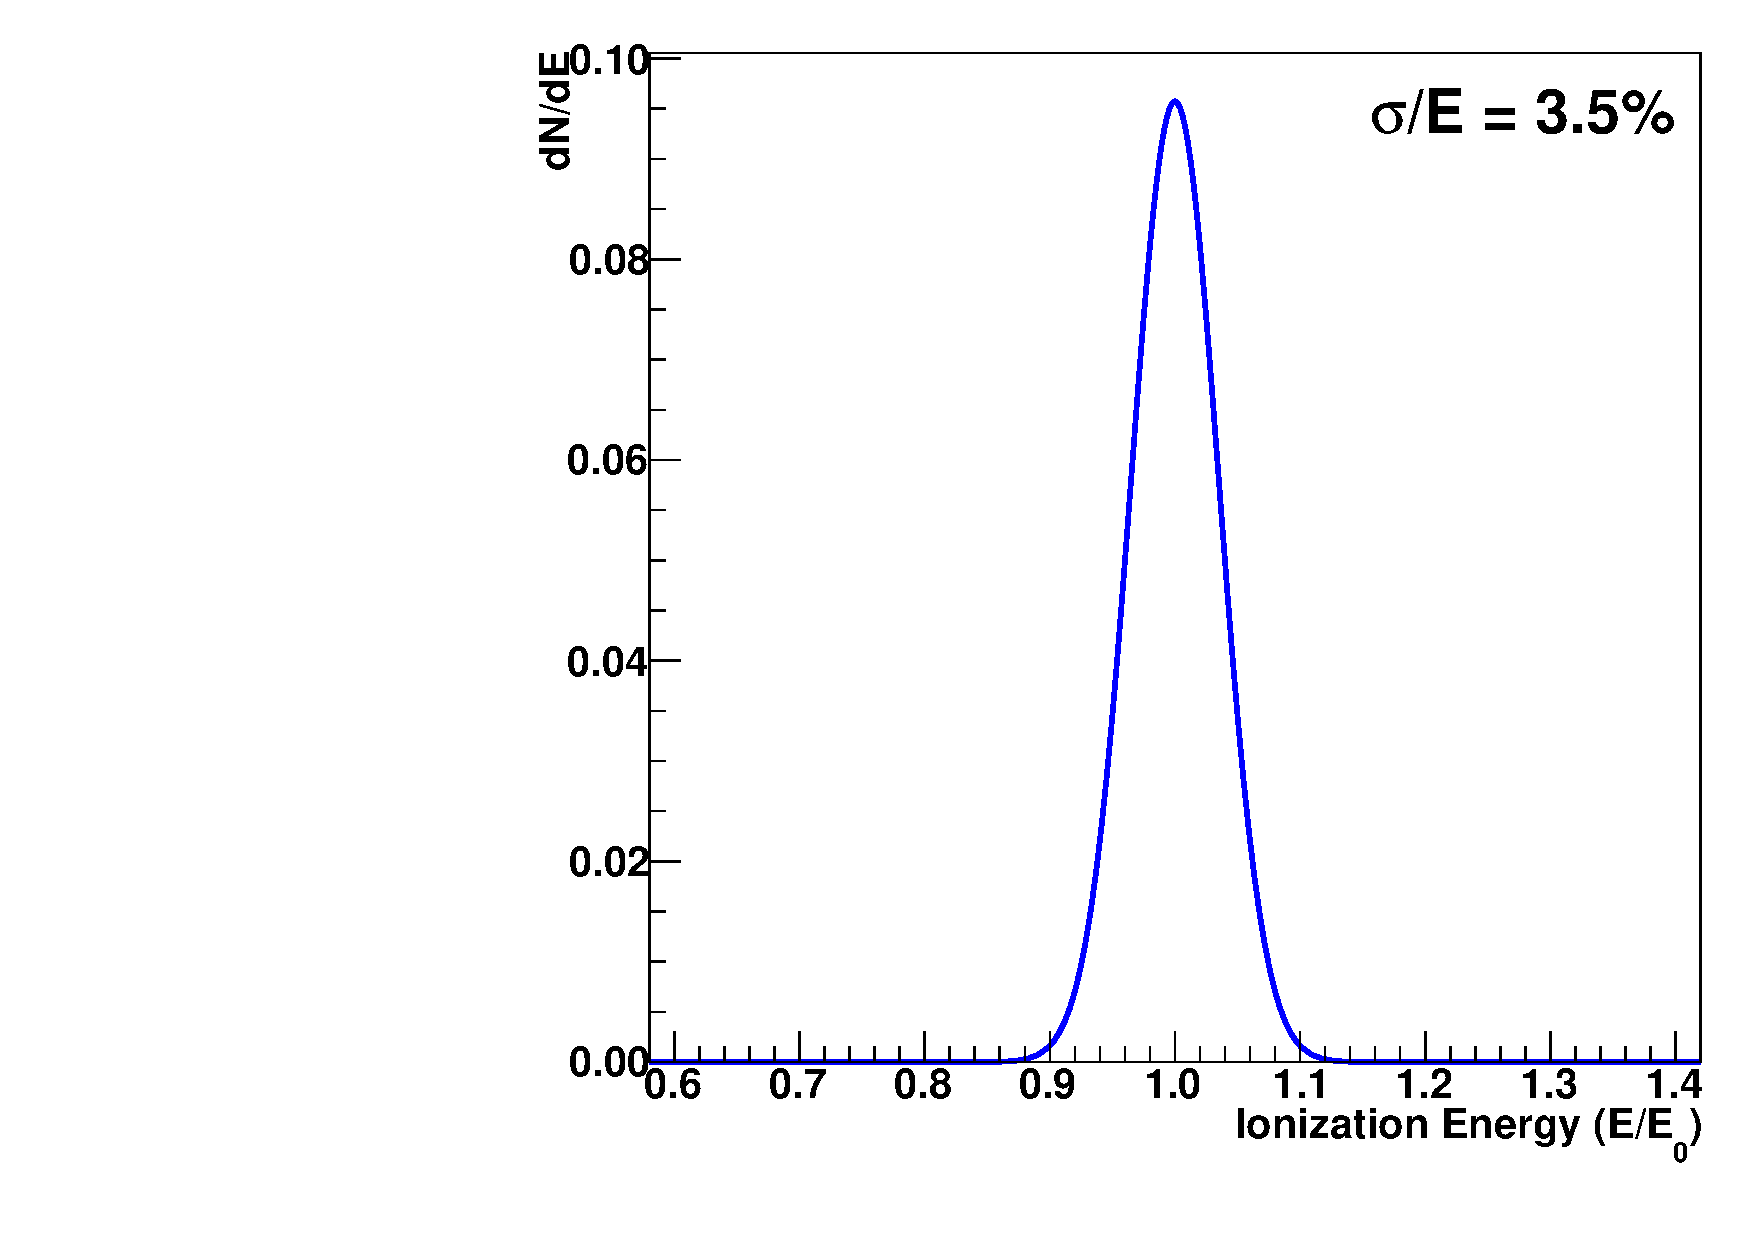
\includegraphics[width=\textwidth]{./plots/xe_anticorrelation_ioniz.pdf}
\end{subfigure}\hspace{0.05\linewidth}\hfill%
\begin{subfigure}[c]{0.45\linewidth}
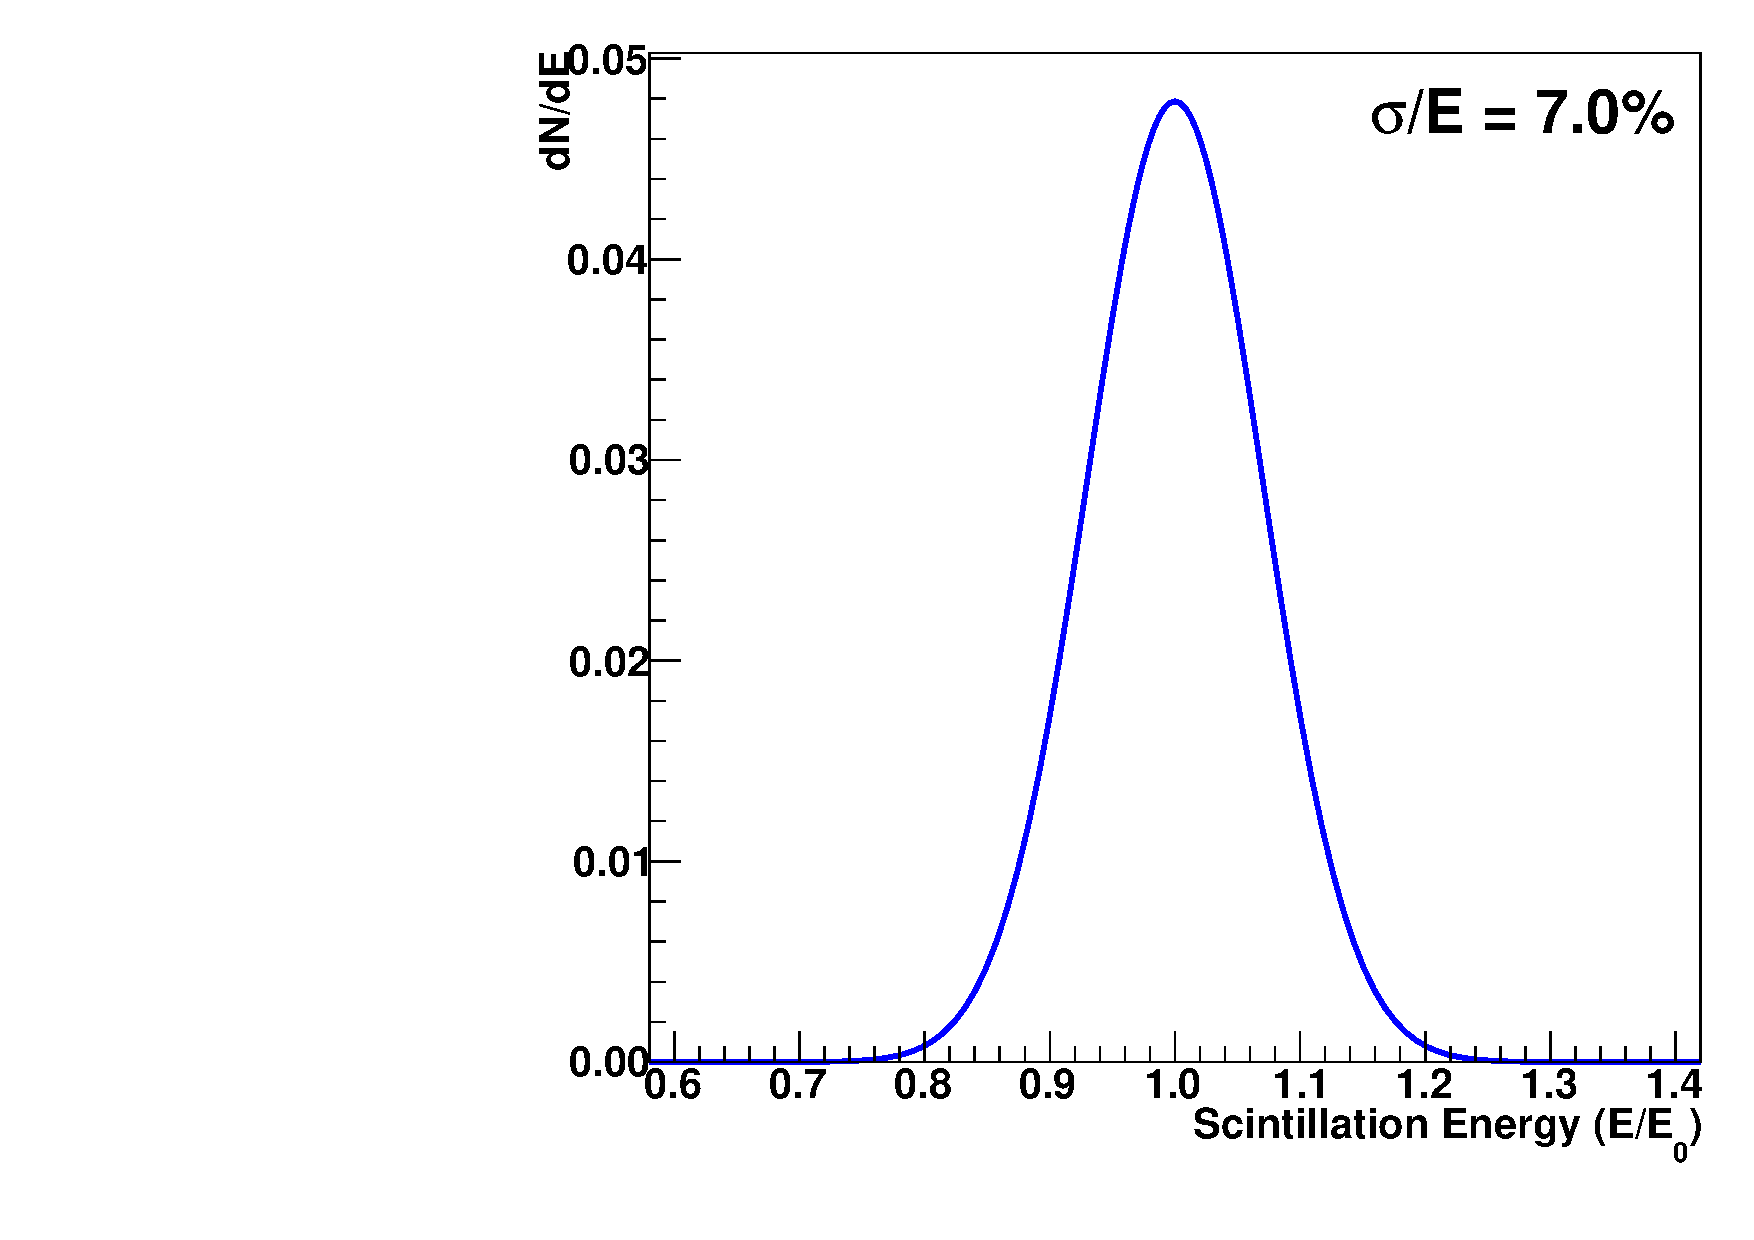
\includegraphics[width=\textwidth]{./plots/xe_anticorrelation_scint.pdf}
\end{subfigure}
\begin{subfigure}[c]{0.45\linewidth}
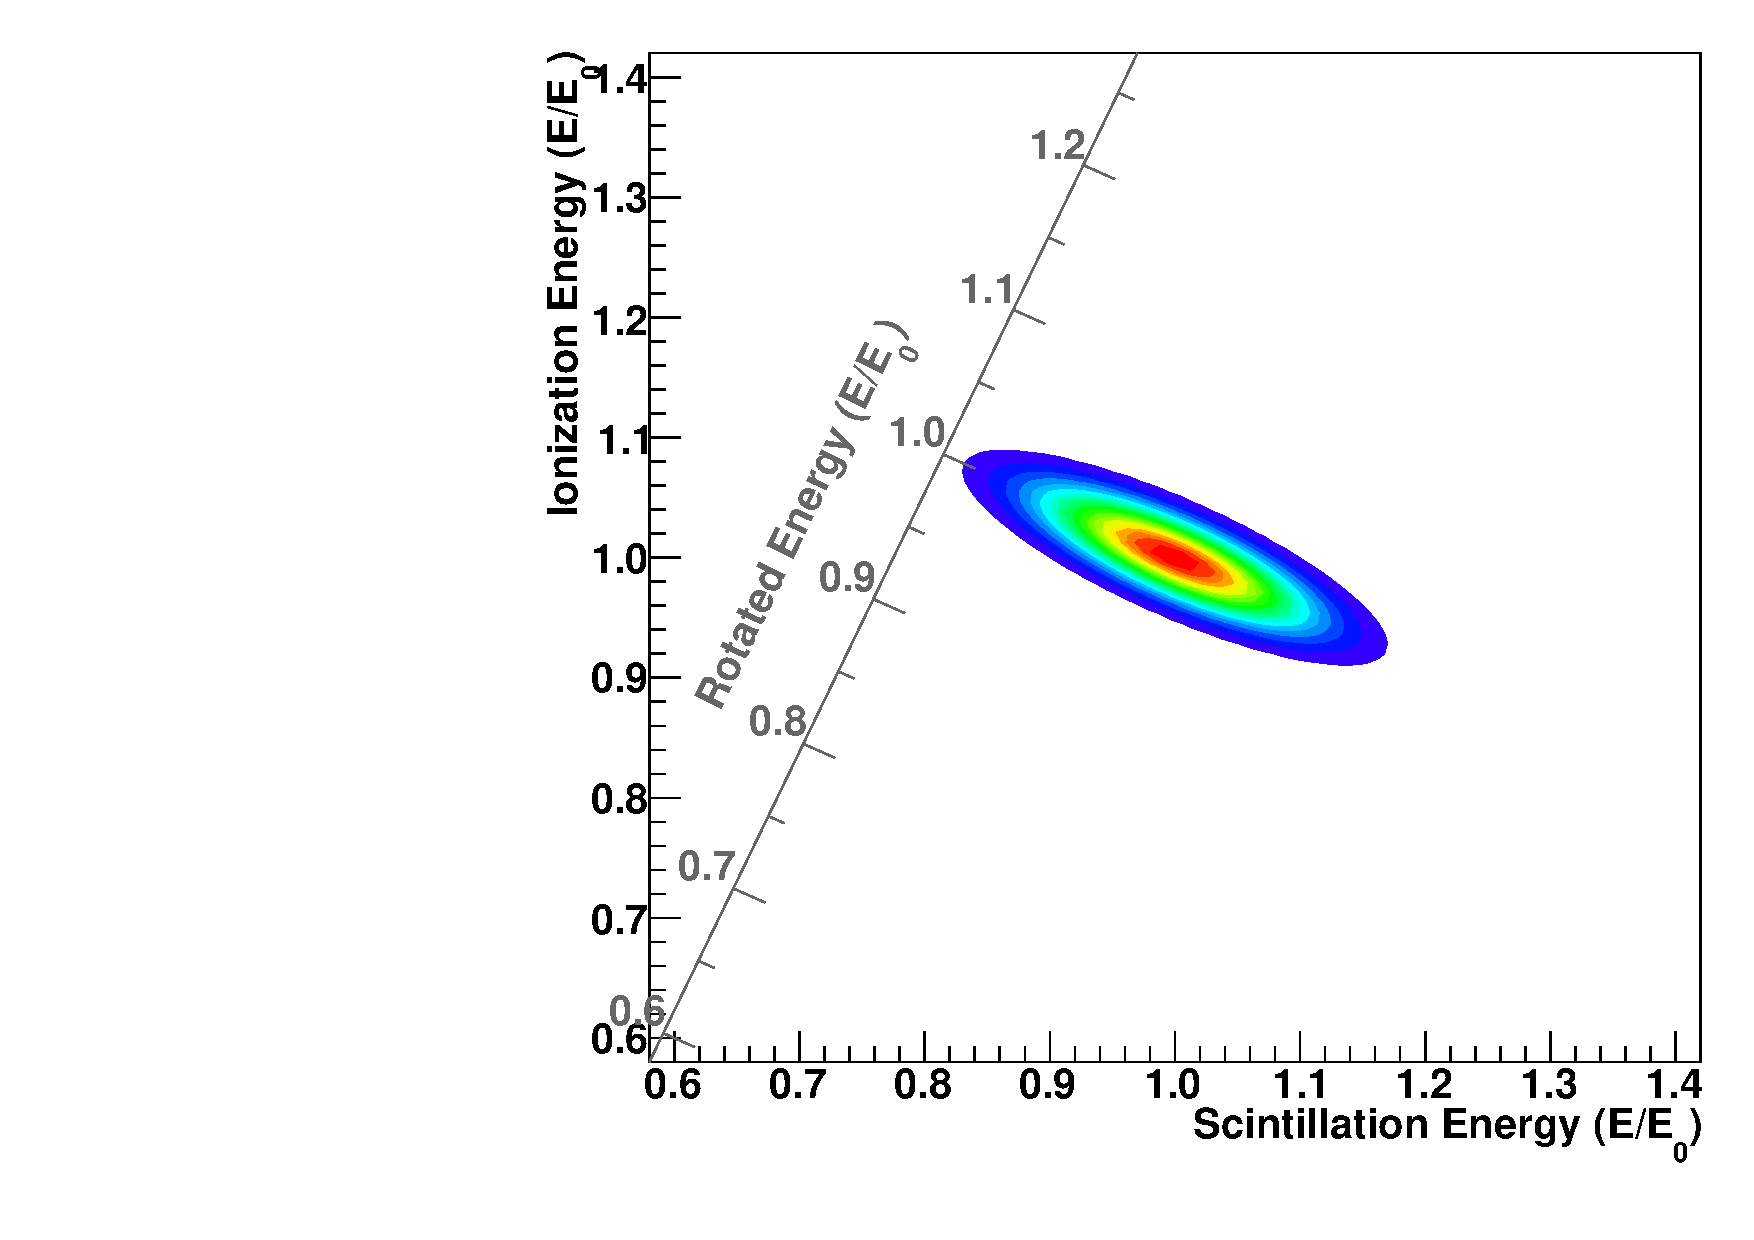
\includegraphics[width=\textwidth]{./plots/xe_anticorrelation_2d.pdf}
\end{subfigure}\hspace{0.05\linewidth}\hfill%
\begin{subfigure}[c]{0.45\linewidth}
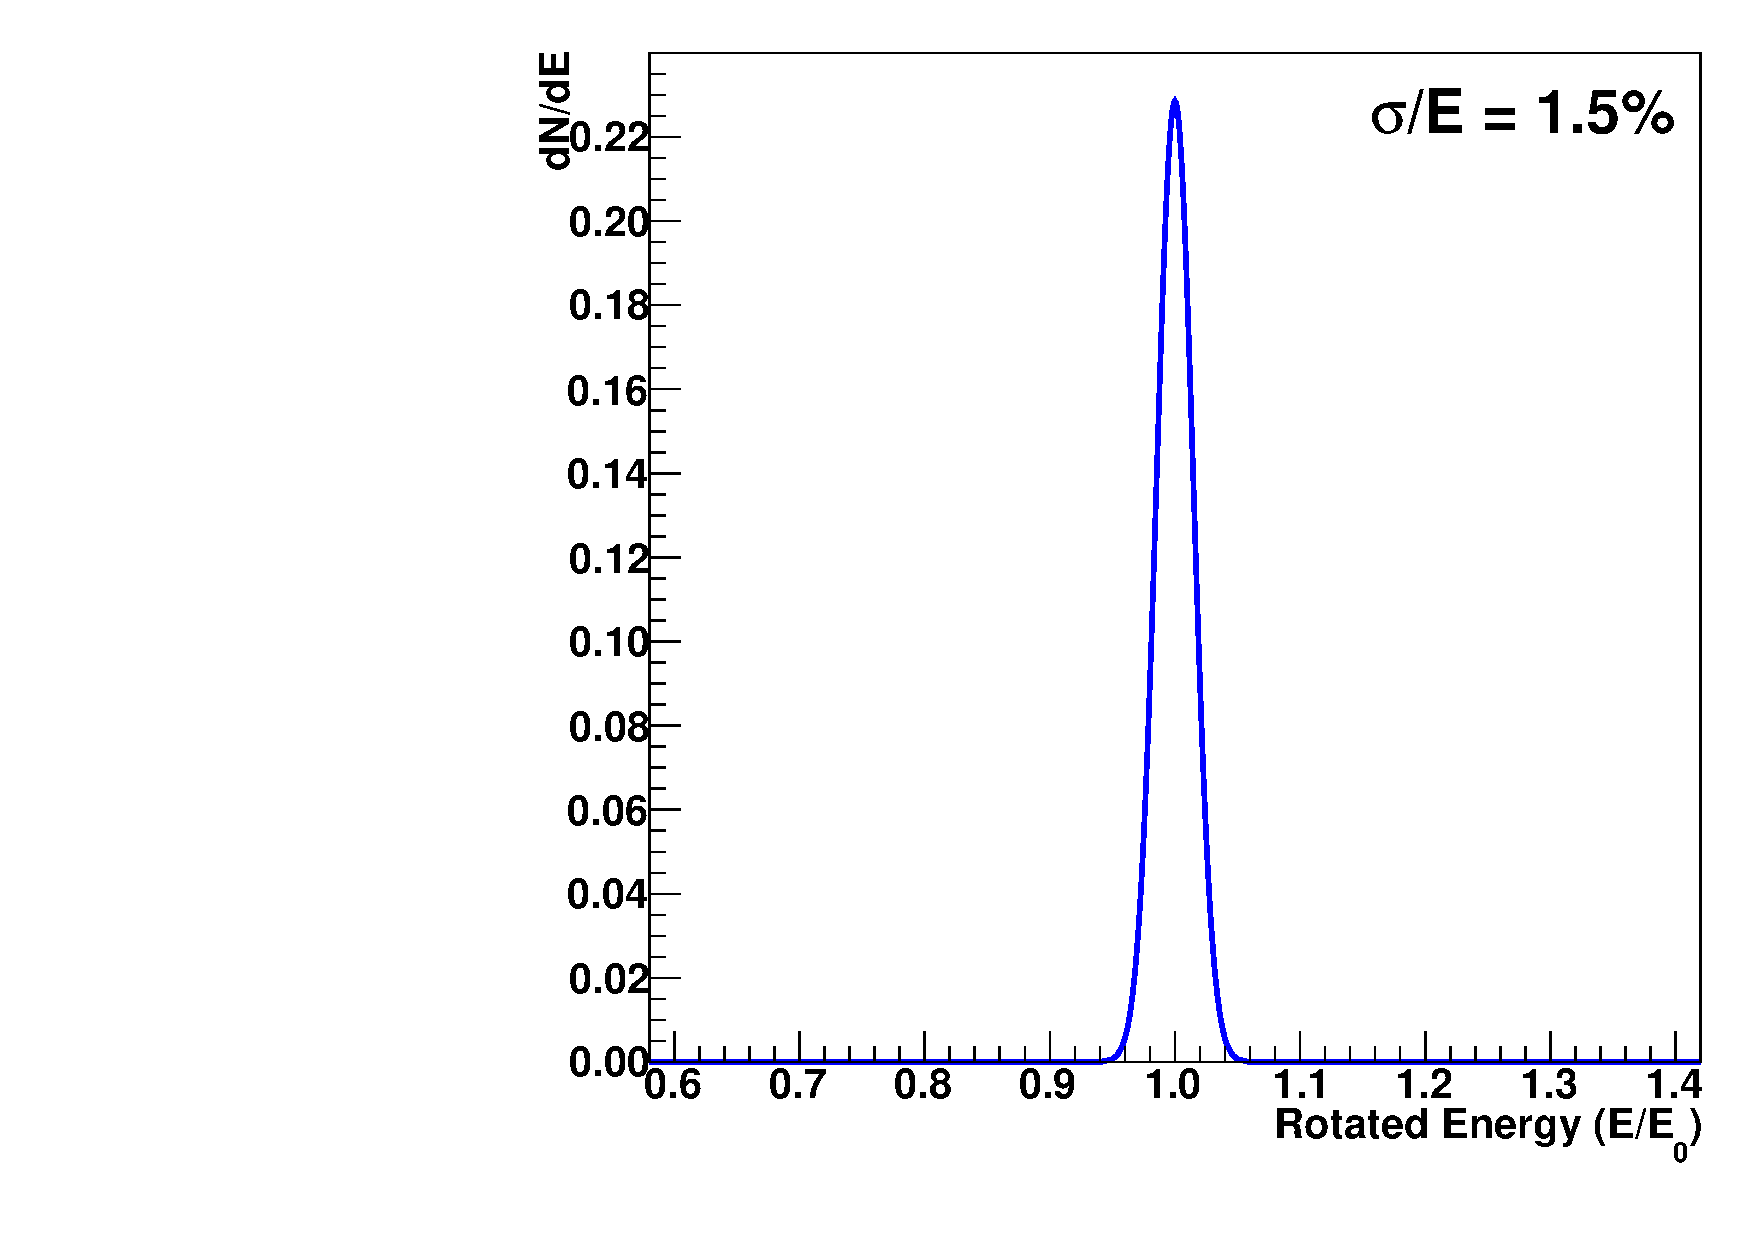
\includegraphics[width=\textwidth]{./plots/xe_anticorrelation_rot.pdf}
\end{subfigure}
\caption[Combining signals to improve energy resolution in liquid xenon]{A toy example of how the energy resolution of a monoenergetic line can be improved by combining signals in liquid xenon. The ionization signal (top left) and the scintillation signal (top right) show poor energy resolution individually. When the signals are anticorrelated (shown bottom left, with coefficient -0.8), they can be protected onto a rotated axis to yield an improved energy resolution (bottom right).}
\label{fig:xe_toy_anticorrelation}
\end{figure}

Electron-ion pairs can recombine to produce one scintillation photon. The probability for this to occur depends both on the ionization density and the strength of the electric field applied. A stronger field will cause more electrons to drift away from the ions before they can recombine. Particles such as \(\alpha\) particles that are highly ionizing create a higher ionization density, and so an increased ratio of scintillation to ionization can be used to distinguish them from \(\beta\) and \(\gamma\) radiation. While the recombination of ions to produce scintillation can be modeled \cite{Doke:1988qf,Thomas:1987ve}, collecting both ionization and scintillation signals allows an unambiguous measurement of the total energy deposited in the detector.

A toy example of combining the ionization and scintillation signals is shown in \cref{fig:xe_toy_anticorrelation}. Even assuming a less-than-perfect correlation between ionization and scintillation due to effects such as imperfect collection and detector noise, this example shows how combining the signals can yield a dramatic improvement in resolution. This has been demonstrated to work in practice \cite{Conti:2003tg,Aprile:2007hc}. However, the energy resolution for the combined signals in such experiments still falls short of the Poisson limit, suggesting other factors contribute to worsening the energy resolution in liquid xenon.

\section{Radiopurity}
Liquid xenon is dense (\about~\SI{3}{\g\per\cubic\cm}) and has a high atomic number (\(Z=54\)). It provides good shielding against low-energy \(\gamma\) rays from external sources. The attenuation length of a \SI{100}{keV} photon is less than \SI{2}{\mm} \cite{Berger:2010dq}. However, this shielding grows worse for higher-energy photon. A \SI{1}{MeV} photon has an attenuation length of nearly \SI{6}{\cm}, and so the self-shielding begins to become less useful for a double beta decay search.

Since xenon is a noble gas, nearly all internal radioactive contaminants can be removed chemically. However isotopes of other noble elements like \isotope{85}{Kr} (a \(\beta^{-}\) emitter primarily produced as a byproduct to nuclear fission), \isotope{222}{Rn}, and \isotope{220}{Rn} (naturally occurring due to \ce{U} and \ce{Th} decays) are potential trace backgrounds. Krypton can be removed through distillation or ultracentrifugation. Since many decays occur along the full radon chains, there is some potential to tag radon daughter decays, especially making use of the \(\alpha\) particle identification described above in \cref{sec:xe_combining_ion_and_scint}. Cosmogenic \xenon{135} and \xenon{137} can be mitigated by a rock overburden to provide shielding from cosmic rays, and are in any case short-lived.

Standard double beta decays will always be a background, of course, to searches for other modes. Precise measurements of the standard mode's half-life will make excesses due to nonstandard modes more significant. Good energy resolution, meanwhile, can improve the discrimination between the modes.
\end{document}
